\subsection{Sign Up}
\label{ssec:konzept:client:signup}
Die Registrierung im System ermöglicht es einem Nutzer, eigene Umfragen erstellen zu können.
Um einen neuen Account anzulegen, muss der Nutzer, wie in Abbildung~\ref{fig:MockSignup} dargestellt, seinen gewünschten Benutzernamen, seine E-Mail-Adresse sowie sein gewünschtes Passwort in die zugehörigen Eingabefelder eingeben.
Durch das wiederholte Eingeben des Passwortes sollen eventuelle Fehler beim Eintippen verhindert werden.
Daraus folgend werden Supportanfragen bezüglich des Passwortes stark reduziert.

\begin{figure}[H]
	\centering
	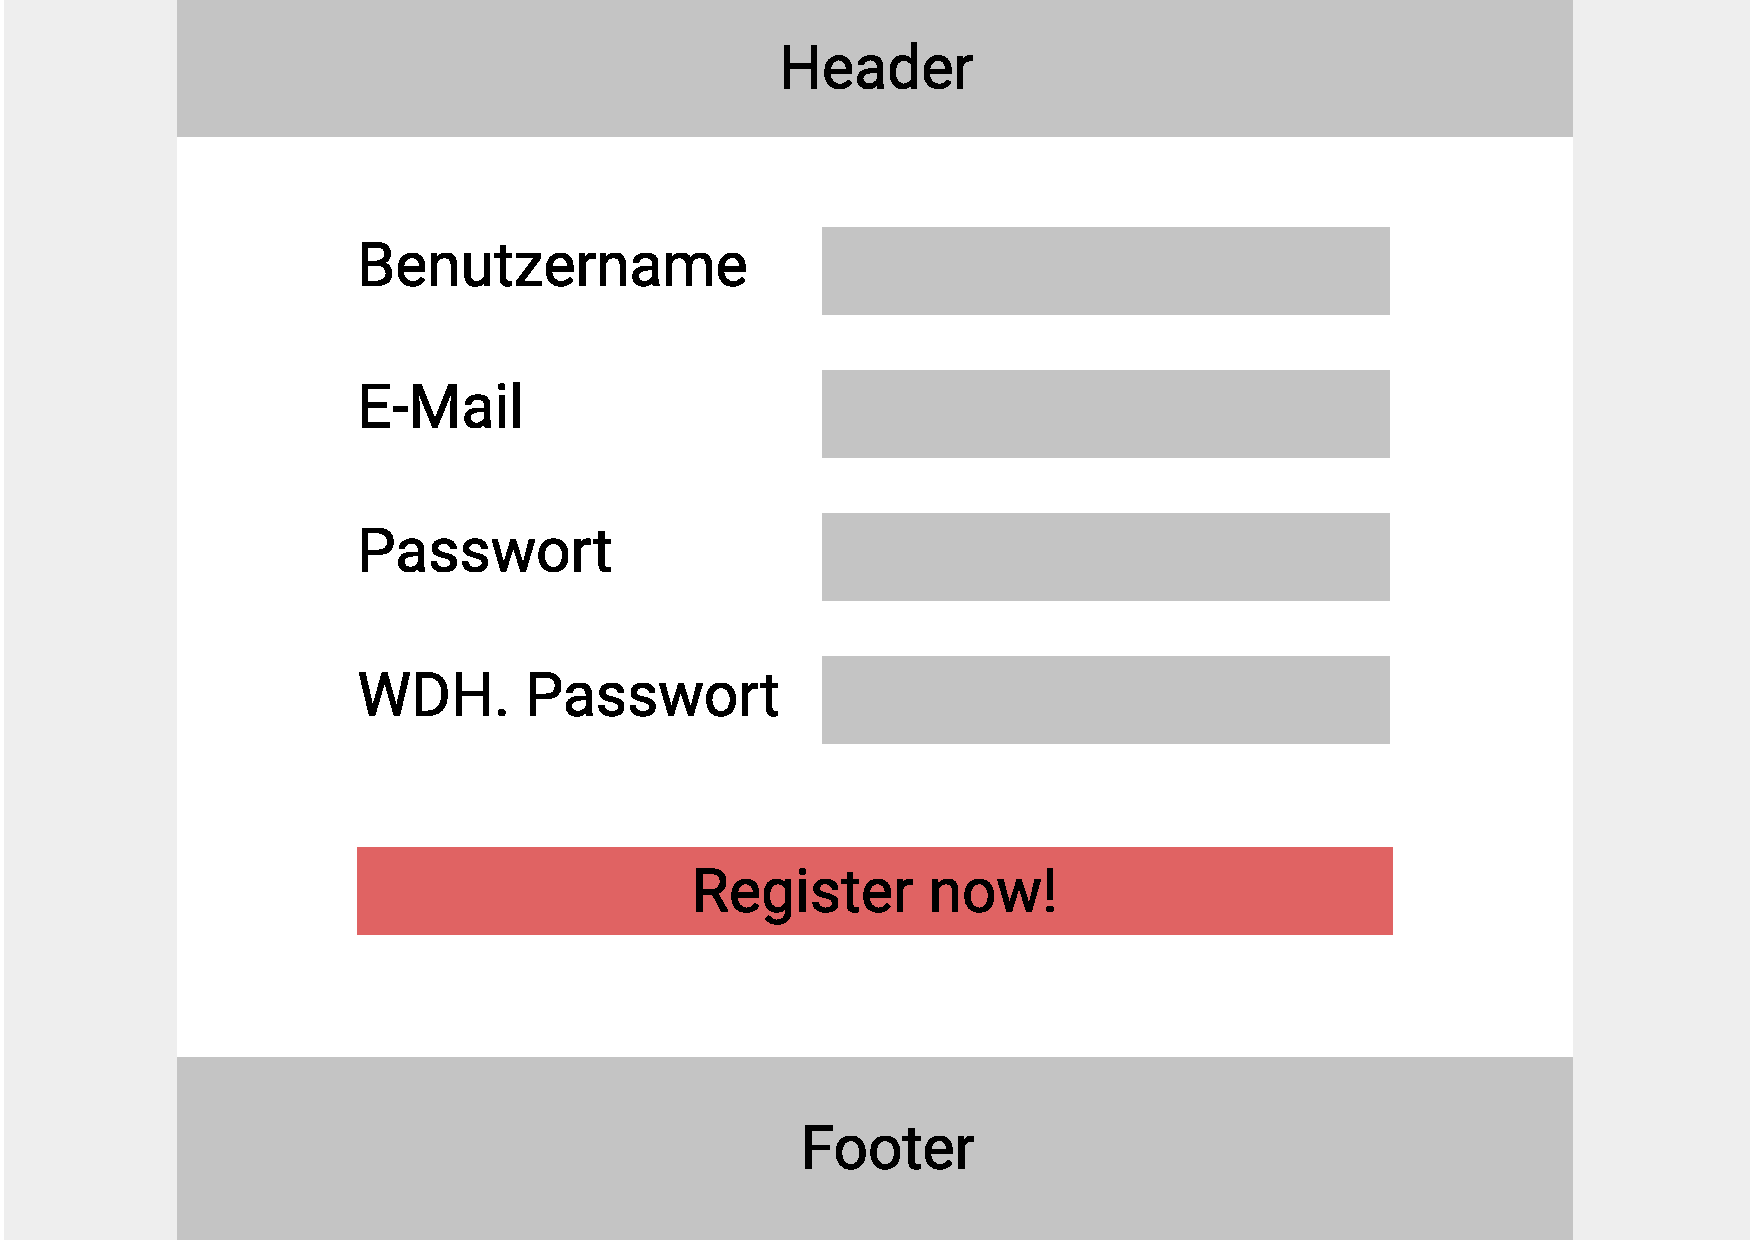
\includegraphics[width=0.7\textwidth]{img/konzeption/client/register}
	\captionsetup{justification=centering, format=plain}
	\caption[Mock-Up der Registrierungsseite]{Mock-Up der Registrierungsseite \\\figma}
	\label{fig:MockSignup}
\end{figure}
